\chapter{LaTeX}

In this LaTex further reading exercise we will be discussing the data obtained from the various websites proposed. Most of this information is based on personal opinions, but to some extent they have a very solid justification.

Many of these resources provide comparisons with other text processing tools such as MS Word or OpenOffice Writer. On the following table we show a summary of the sources visited\footnote{https://www.http://openwetware.org/wiki/Word_vs._LaTeX.org/conference/lisa12/technical-sessions/presentation/weaver}.\footnote{http://tex.stackexchange.com/questions/1756/why-should-i-use-latex}

{
\centering
\begin{tabular}{l | p{8cm}}
Characteristic & Differences \\ \hline
\texttt Small, simple documents & For these kind of documents, regular text editors tend to perform better as they have almost no learning time. These kind of documents often do not need the features LaTeX provides. \\ \hline
\texttt Ease of use & Most text processing programs are really easy to use nowadays, and a writer can adapt from one to another in little time. LaTeX however, requires some degree of knowledge of it's non-trivial commands, which makes it a little harder to learn.  \\ \hline
\texttt Scientific Writing & This is one of the fields where LaTeX outshines text editors. It has special features that allow for this kind of documents (heavy on formulas or graphics) to be written with less effort and in a more consistent way.  \\ \hline
\texttt Layout & LaTeX shines again in this characteristic. While text editors often come with functionality to define the layout of the documents, they are not nearly powerful as LaTeX tools for that purpose.  \\ \hline
\end{tabular}
}



\section{Conclusions}
\label{sec:conclusions}

The first idea that comes to mind is that regular text editors are easy to learn and use at first glance. LaTeX powerfulness comes at the cost of having to learn a more complex editing tool, which can be a huge drawback in certain environments. However, after this first difficulties are dealt with, LaTeX can produce higher quality large documents with considerable less effort than the other editors, thanks to it's capability of data and format separation.

A second important conclusion could be the fact that LaTeX is way better prepared to deal with specific types of publications that require special writing techniques, such as handling scientific formulas. Regular text editors have some ways to work around that, but the process is much simpler and provides better results on LaTeX.

As a final evaluation, we can say that there is not a single application that can serve all purposes. Both text editing tools and LaTeX have their own strong and weak points, and it's up to the final user/editor to choose the correct one for his project.

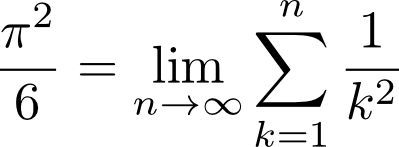
\includegraphics[scale=0.5]{Chapters/LatexFormulaEffect.png}
